\documentclass[12pt, a4paper]{article}
\usepackage[utf8]{inputenc}
\usepackage[russian]{babel}
\usepackage[pdftex]{graphicx, color}
\usepackage{amsmath, amsfonts, amssymb, amsthm, mathrsfs}
\usepackage[left=2cm,right=2cm,top=1.5cm,bottom=2cm]{geometry}
\usepackage{indentfirst}

\usepackage{setspace}
\onehalfspacing
\graphicspath{{pics/}}

\begin{document}

    \thispagestyle{empty}

    \begin{singlespace}
    \begin{titlepage}
        \begin{center}
            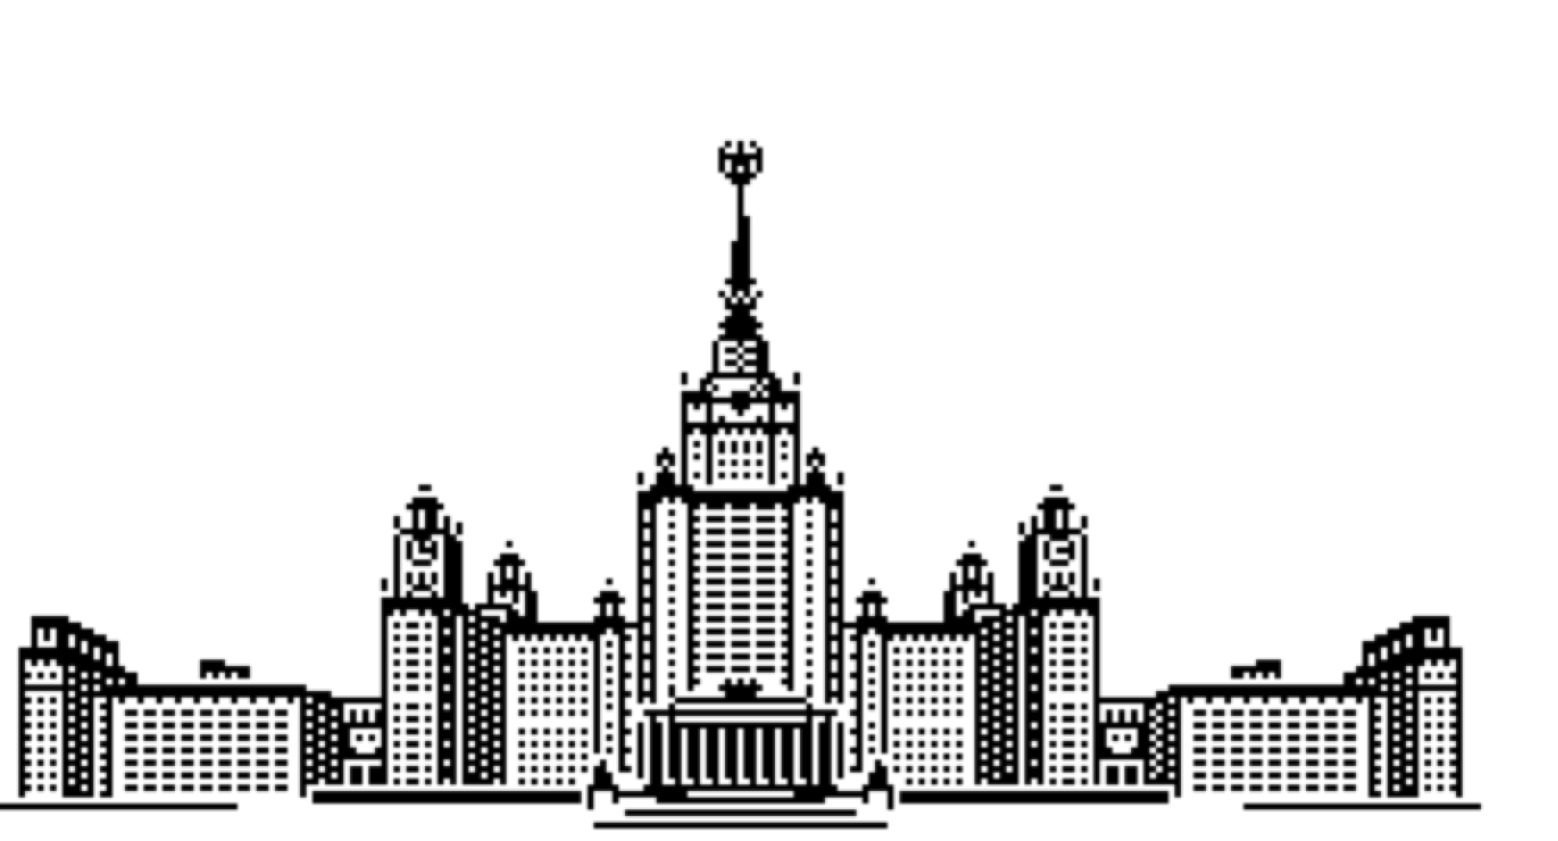
\includegraphics[height = 3cm]{msu.png}

            {\scshape Московский государственный университет имени М.~В.~Ломоносова}\\
            Факультет вычислительной математики и кибернетики\\
            Кафедра математических методов прогнозирования\\
            \centerline{\hfill\hrulefill\hrulefill\hrulefill\hrulefill\hfill}

            \vfill

            {\Large \textit{Аят Оспанов}}

            \vspace{1mm}

            {\LARGE Современные подходы в задачах NLP:\\
            <<Система нейронного машинного перевода от Google: преодоление разрыва между человеческим и машинным переводом>>}


        \end{center}

        \vfill
        \vfill

        \begin{center}
            Москва, 2017
        \end{center}
    \end{titlepage}
    \end{singlespace}

    \newpage
    \tableofcontents

    \newpage
    \section{Введение}
        Нейронный машинный перевод (NMT, англ. Neural Machine Translation) был недавно представлен как многообещающий подход с возможностью устранения многих недостатков традиционных систем машинного перевода. Мощь NMT заключается в его способности непосредственно учиться отображению входного текста в соответствующий выходной текст. Его архитектура, как правило, состоит из двух рекуррентных нейронных сетей (RNN), одна из которых предназначена для использования входной текстовой последовательности, а другая для генерации переведенного выходного текста. NMT часто сопровождается механизмом внимания, который помогает эффективно справляться с длинными входными последовательностями.

        Преимущество NMT заключается в том, что он обходит многие хрупкие варианты дизайна в традиционном машинном переводе на основе фраз. Однако на практике системы NMT были менее точны по сравнению с системами перевода на основе фраз, особенно при обучении очень большим наборам данных, которые используются в самых лучших общедоступных системах перевода. За этот пробел отвечают три недостатка, присущие NMT: его медленное обучение и скорость вывода, неэффективность в работе с редкими словами, а иногда и невозможность перевести все слова в исходном предложении. Во-первых, для обучения NMT-системы в большом наборе переводов обычно требуется значительный объем времени и вычислительных ресурсов, что замедляет скорость экспериментальных открытий и инноваций. Как правило, они гораздо медленнее, чем системы на основе фраз из-за большого количества используемых параметров. Во-вторых, NMT не хватает надежности перевода редких слов. Хотя это можно решить путем обучения «модели копирования» для имитации традиционной модели выравнивания или использования механизма внимания для копирования редких слов. Оба этих подхода являются ненадежными в масштабе, поскольку качество выравнивания в разных языках различаются, а скрытые выравнивания, созданные механизмом внимания, нестабильны для глубоких сетей. Кроме того, простое копирование не всегда может быть лучшей стратегией для работы с редкими словами, например, когда транслитерация более уместна. Наконец, системы NMT иногда производят выходные предложения, которые не переводят все части входного предложения, другими словами, они не могут полностью «покрыть» входные данные, что может привести к неожиданным переводам.

        В этой работе представлен обзор на Нейронный Машинный Переводчик от Google (GNMT, Google NMT) -- производственной системы NMT в Google, которая направлена на решение вышеприведенных проблем. В реализации Google рекуррентными сетями являются RNN с длинной кратковременной памятью (LSTM, Long Short-Term Memory). LSTM RNN в GNMT имеют 8 слоев, с остаточными связями между слоями для поощрения градиентного потока. Для параллелизма механизм внимания соединяется с нижним уровнем сети декодера и верхним уровнем сети энкодера. Чтобы улучшить время вывода, используется низкоточные арифметические выражения для вывода, которое дополнительно ускоряется специальным оборудованием (Tensor Processing Unit или TPU). Чтобы эффективно работать с редкими словами, используется подсловные единицы (также известные как <<wordpieces>>) для входов и выходов в системе. Использование «wordpieces>> дает хороший баланс между гибкостью отдельных символов и эффективностью полных слов для декодирования, а также обходит необходимость специальной обработки неизвестных слов. <<Метод поиска луча>> (Beam search technique) включает процедуру нормализации длины для эффективного решения проблемы сравнения гипотез разной длины при декодировании и штраф за покрытие способствующий модели для перевода всех предоставленных входных данных.

    \section{Архитектура модели}
        Модель (см. Рис. \ref{fig:arch}) следует общей схеме обучения <<от последовательности к последовательности>> (sequence-to-sequence) с вниманием. Она состоит из трех компонентов: сети энкодера, сети декодера и сети внимания. Энкодер преобразует исходное предложение в список векторов; один вектор на входной символ. Учитывая этот список векторов, декодер производит по одному символу за раз, пока не будет создан специальный символ конца предложения (EOS). Энкодер и декодер соединены через модуль внимания, который позволяет декодеру фокусироваться на разных регионах исходного предложения во время декодирования.

        Для обозначения используется: жирный нижний регистр для векторов (например, $\mathbf{v}, \mathbf{o_i}$), жирный верхний регистр для представления матриц (например, $\mathbf{U}, \mathbf{W}$), верхний регистр курсивом для представления множеств (например, $\mathscr{V}, \mathscr{T}$), прописные буквы для представления последовательностей (например, $X, Y$) и нижний регистр для представления отдельных символов в последовательности (например, $x_1, x_2$).

        Пусть $(X, Y)$ -- пара исходного и целевого предложения. Пусть $X = x_1, x_2, x_3, \dots, x_M$ -- последовательность из $M$ символов в исходном предложении, и пусть $Y = y_1, y_2, y_3, \dots, y_N$ -- последовательность из $N$ символов в целевом предложении. Тогда энкодер -- эта функция следующего вида:

        \begin{equation}
            \mathbf{x_1, x_2, \dots, x_M} = \textit{EncoderRNN}(x_1, x_2, x_3, ..., x_M)
        \end{equation}

        В этом ураавнении $\mathbf{x_1, x_2, \dots, x_M}$ -- список векторов одинакового фиксированного размера. Число членов в списке такое же, как количество символов в исходном предложении (в этом примере $M$). Используя цепное правило (chain rule), условную вероятность последовательности $P(Y|X)$ можно разложить как:

        \begin{equation}
            P(Y|X) = P(Y|\mathbf{x_1, x_2, x_3, \dots, x_M}) = \prod_{i=1}^{N}P(y_i|y_0, y_1, y_2, \dots, y_{i-1};\mathbf{x_1, x_2, x_3, \dots, x_M})
        \end{equation}

        Таким образом во время вывода вычисляется вероятность следующего символа с учетом кодированного исходного предложения и декодированной последовательности:
        \begin{equation}
            P(y_i|y_0, y_1, y_2, \dots, y_{i-1};\mathbf{x_1, x_2, x_3, \dots, x_M})
        \end{equation}

        Декодер реализован как комбинация сети RNN и слоя softmax. Сеть RNN декодера создает скрытое состояние $y_i$ для следующего прогнозируемого символа, который затем проходит через слой softmax для генерирования распределения вероятности по выходным символам-кандидатам.

        По проведенным экспериментам выяснилось, что системы NMT должны иметь достаточно глубокие RNN энкодеры и декодеры чтобы выявить тонкие неровности в исходных и целевых языках. В этой модели каждый добавленный слой уменьшал перплексию на около 10\%. В рассматриваемом методе используется глубокие LSTM сети и для RNN-энкодера и для RNN-декодера.

        Модуль внимания в данной сети похож на модуль внимания из сети, представленной в \cite{nmt}. Более конкретно, пусть $y_{i-1}$ -- это выход RNN-декодера из предыдущего шага декодирования. Контекст внимания $a_i$ для текущего временного шага вычисляется по следующим формулам:
        \begin{equation}
        \begin{aligned}
            s_t &= \textit{AttentionFunction}(y_{i-1}, x_t) \quad \forall t, \quad 1 \leq t \leq M \\
            p_t &= \text{exp}(s_t) / \sum_{t=1}^{M} \text{exp}(s_t) \quad \forall t, \quad 1 \leq t \leq M \\
            a_i &= \sum_{t=1}^{M}p_t \cdot \mathbf{x_t}
        \end{aligned}
        \end{equation}
        где $AttentionFunction$ -- сеть прямого распространения с одним скрытым слоем.

        \begin{figure}
            \centering
            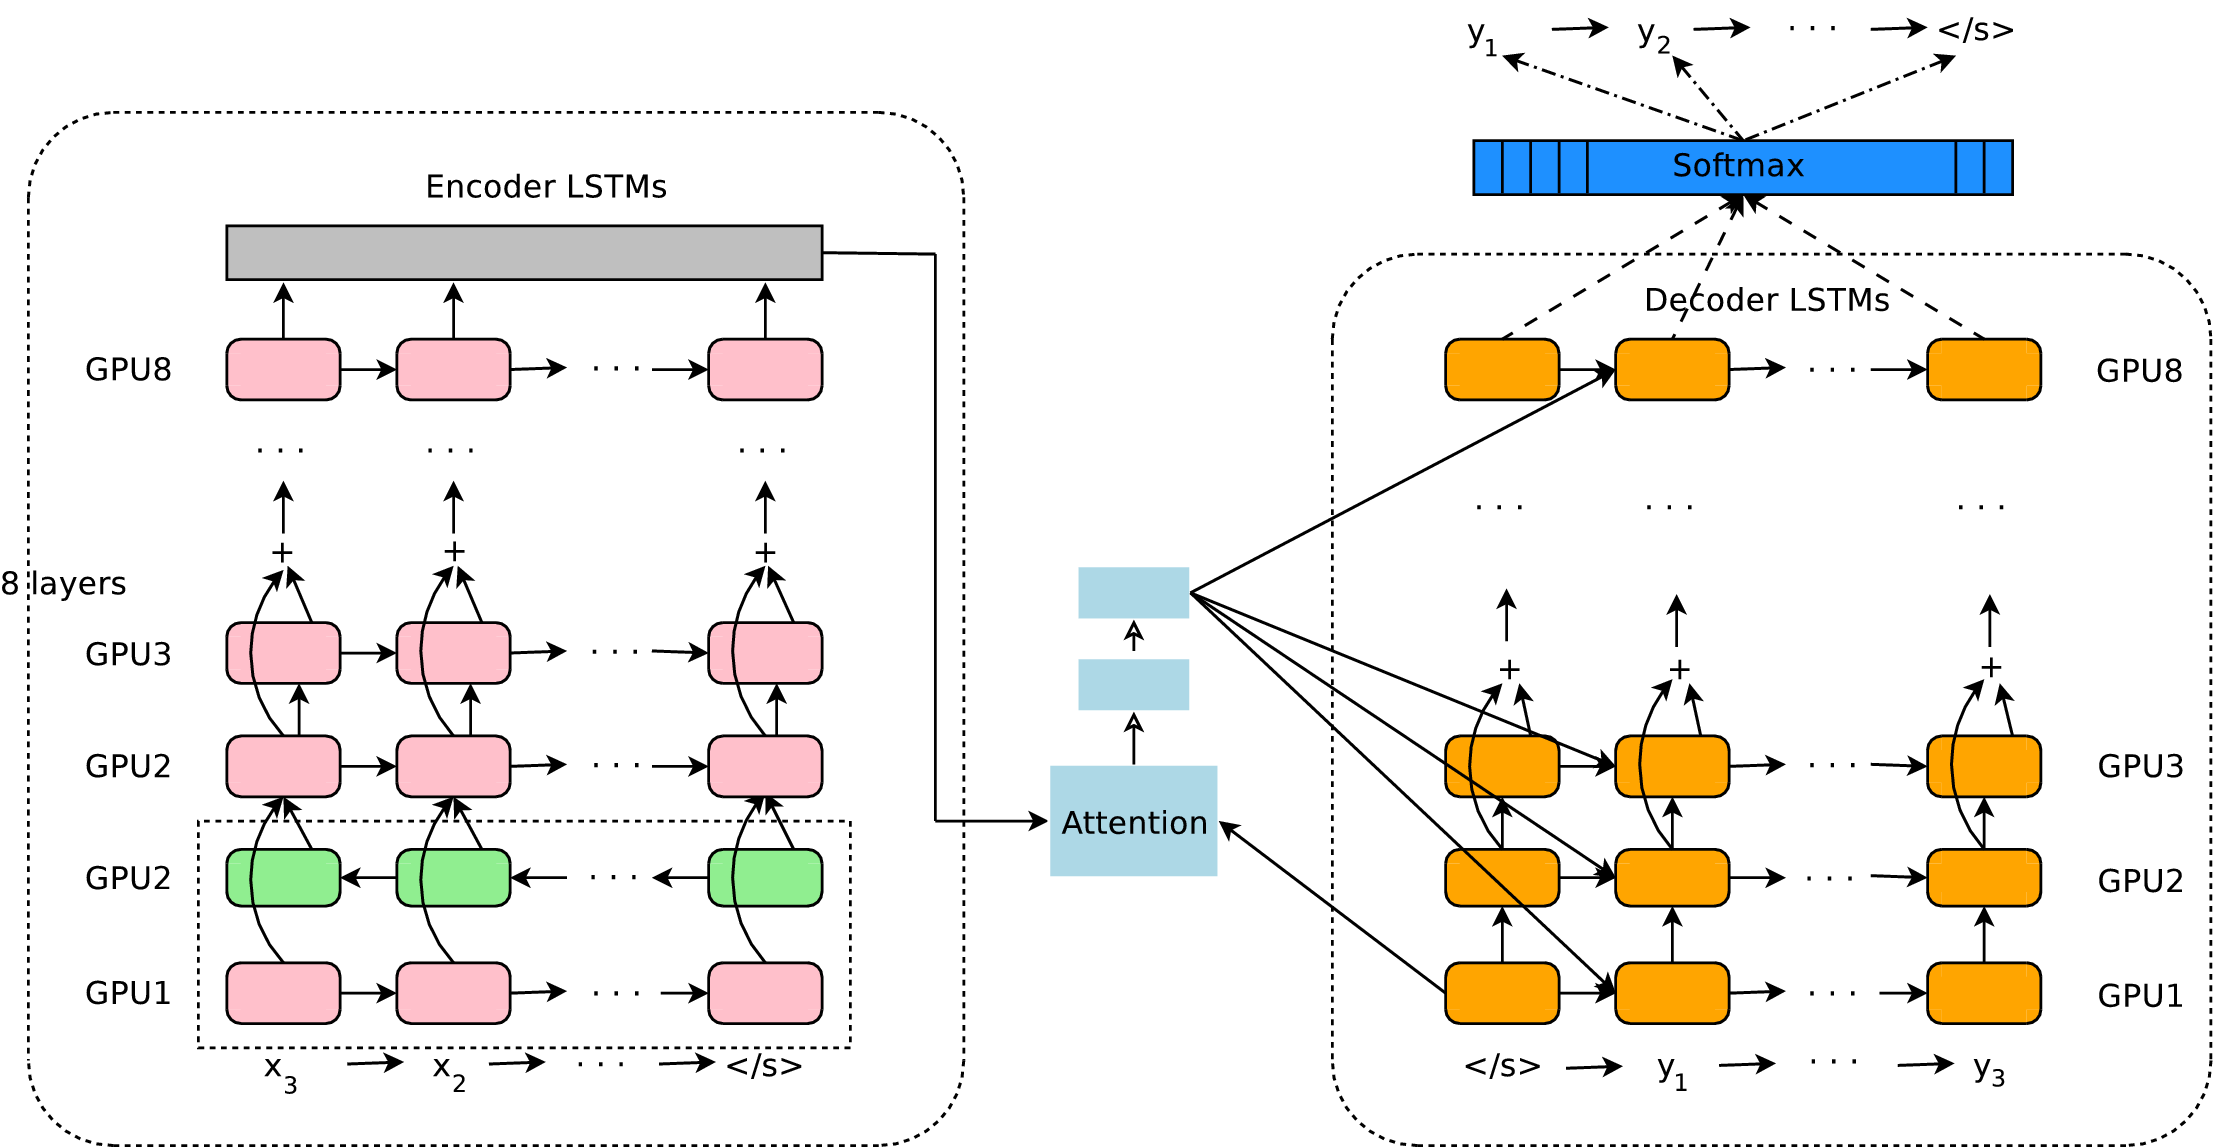
\includegraphics[width=\textwidth]{arch.png}
            \caption{Модельная архитектура GNMT, системы Neural Machine Translation от Google. Слева -- сеть энкодера, справа -- сеть декодера, посередине -- модуль внимания. Нижний слой кодировщика двунаправлен: розовые узлы собирают информацию слева направо, а зеленые узлы собирают информацию справа налево. Другие слои энкодера являются однонаправленными. Остаточные соединения начинаются с третьего слоя снизу в энкодере и декодере.}
            \label{fig:arch}
        \end{figure}

    \section{Модель Wordpiece}
        Модели нейронного машинного перевода часто работают со словарями с фиксированным количеством слов, хотя перевод -- это в основном открытая проблема лексики (имена, числа, даты и т.д.). Существует две широкоиспользуемых категорий подходов к переводу слов-вне-словаря (OOV, англ. out-of-vocabulary). Один из подходов состоит в том, чтобы просто копировать редкие слова из источника в перевод (поскольку большинство редких слов -- это имена или числа, где правильный перевод -- это просто копия) либо на основе модели внимания, используя внешнюю модель выравнивания. Или даже используя более сложную целевую сеть специального назначения. Другой категорией подходов является использование подсловных единиц (sub-word units), например символов, смешанного слова/символов или более умно подобранных подслов.

        Наиболее успешный подход относится ко второй категории (подсловные единицы), и Google применяет реализацию модели Wordpiece (WPM), изначально разработанную для решения проблемы сегментации японского и корейского языков для системы распознавания речи Google. Этот подход полностью управляется данными и гарантированно генерирует детерминированную сегментацию для любой возможной последовательности символов. Он аналогичен методу, использованному в \cite{subword}, для обработки редких слов в NMT.

        Для обработки произвольных слов сначала слова разбиваются на wordpiece-ы, полученные с помощью обученной wordpiece модели. Специальные символы границы слова добавляются перед обучением модели, так что первоначальная последовательность слов может быть восстановлена из последовательности wordpiece-ов без двусмысленности. Во время декодирования модель сначала создает последовательность wordpiece-ов, которая затем преобразуется в соответствующую последовательность слов.

        Ниже приведен пример последовательности слов и соответствующей последовательности wordpiece-ов:
        \begin{itemize}
            \item \textbf{word}: Jet makers feud over seat width with big orders at stake
            \item \textbf{wordpiece}: \_J et \_makers \_fe ud \_over \_seat \_width \_with \_big \_orders \_at \_stake
        \end{itemize}

        В приведенном выше примере слово ``Jet'' разбито на два слова ``\_J'' и ``et'', а слово ``feud'' разбито на два слова ``\_fe'' и ``ud''. Остальные слова остаются как есть. ``\_'' -- специальный символ, добавленный для индикации начала слова.

        Как упоминалось выше, в переводе часто имеет смысл копировать редкие имена или номера объектов непосредственно из источника в перевод. Чтобы облегчить этот тип прямого копирования, всегда используется общаяы модель wordpiece для исходного языка и целевого языка. Использвание этого подхода гарантирует, что одна и та же строка в исходном и целевом предложениях будет разбита на сегменты точно таким же образом, что упростит обучение системы на копирование этих токенов.

        Wordpieces достигают баланса между гибкостью символов и эффективностью слов. Использование wordpiece-ов увеличивает общее количество баллов BLEU для используемых моделей -- возможно, из-за того, что модели теперь эффективно работают с бесконечным словарем, не прибегая к использованию одних только символов. В последнем случае средняя длительность входных и выходных последовательностей будет намного больше и, следовательно, потребуется больше вычислений.

    \section{Тестирование на реальных данных}
        В Google решили протестировать модель на реальных данных. Для этого они попросили людей оценить три типа перевода по шкале от 0 (полная чушь) до 6 (идеальный перевод): 1) перевод системы PBMT (машинный перевод основанный на фразах) использовавшейся в Google, 2) перевод системы GNMT, 3) перевод людей, свободно разговаривающих на обоих языках. В таблице \ref{table:trans_test} представлены средние оценки для переводов Английский $\leftrightarrow$ Французский, Английский $\leftrightarrow$ Испанский, Английский $\leftrightarrow$ Китайский. Все GNMT модели использовали модель wordpiece c 32000 wordpiece-ами. В результате видно, что модель GNMT в большинстве случаев на 60\% уменьшает ошибку перевода по сравнению с PBMT. Распределние оценок показано на Рис. \ref{fig:hist}.

        \begin{figure}
            \centering
            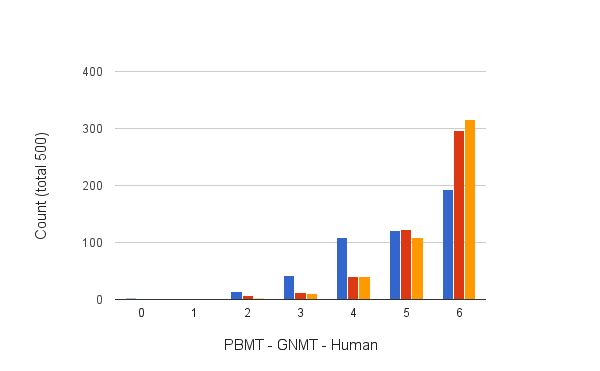
\includegraphics[width=0.8\textwidth]{hist.png}
            \caption{Гистограмма оценок на 500 примерах из Википедии и новостных сайтов для перевода Английский $\rightarrow$ Испанский. Можно видеть, что существует широкое распределение даже для человеческого перевода, что показывает насколько задача неодназначна. Также ясно, что GNMT намного точнее, чем PBMT}
            \label{fig:hist}
        \end{figure}

        \begin{table}[h!]
        \centering
        \begin{tabular}{l c c c c}
            \hline
            \hline
            & PBMT & GNMT & Человек & Относительное \\
            & & & & улучшение \\
            \hline
            Английский $\rightarrow$ Испанский & 4.885 & 5.428 & 5.504 & 87\% \\
            Английский $\rightarrow$ Французский & 4.932 & 5.295 & 5.496 & 64\% \\
            Английский $\rightarrow$ Китайский & 4.035 & 4.594 & 4.987 & 58\% \\
            Испанский $\rightarrow$ Английский & 4.872 & 5.187 & 5.372 & 63\% \\
            Французский $\rightarrow$ Английский & 5.046 & 5.343 & 5.404 & 83\% \\
            Китайский $\rightarrow$ Английский & 3.694 & 4.263 & 4.636 & 60\% \\
            \hline
        \end{tabular}
        \caption{Средние оценки переводов}
        \label{table:trans_test}
        \end{table}

    \section{Заключение}
        В этой работе был сделан обзор на систему нейронного машинного перевода от Google. В итоге можно сделать следующие ключевые заключения: 1) модель wordpiece эффективно обрабатывает открытые словари и проблему морфологически богатых языков, повышая качество перевода и скорость вывода, 2) комбинация параллелизма модели и данных может быть использована для эффективного обучения современных NMT-моделей примерно за неделю, 3) квантование модели резко ускоряет вывод перевода, позволяя использовать эти большие модели в развернутой производственной среде, 4) используя сравнение переводов людьми как метрику, было показано, что GNMT достигает точности среднестатистического человека, владеющего двумя языками. В частности, GNMT на 60\% уменьшает ошибку перевода по сравнение с PBMT.

    \begin{thebibliography}{1}
        \bibitem{nmt}
        Bahdanau, D., Cho, K., and Bengio, Y. Neural machine translation by jointly learning to align and translate. In International Conference on Learning Representations (2015)

        \bibitem{subword}
        Sennrich, R., Haddow, B., and Birch, A. Neural machine translation of rare words with subword units. In Proceedings of the 54th Annual Meeting of the Association for Computational Linguistics (2016)
    \end{thebibliography}

\end{document}
